\documentclass{article}

\usepackage{graphicx}% Include figure files
\usepackage{dcolumn}% Align table columns on decimal point
\usepackage{bm}% bold math
\usepackage{amsmath}
\usepackage{ifthen}
\usepackage{amsfonts}
\usepackage{dsfont}
\usepackage{boxedminipage}
\usepackage{hyperref}
\usepackage{placeins}

\newcommand{\R}{\ensuremath{\mathds{R}}}
\newcommand{\C}{\ensuremath{\mathds{C}}}
\newcommand{\Q}{\ensuremath{\mathds{Q}}}
\newcommand{\N}{\ensuremath{\mathcal{N}}}
\newcommand{\Z}{\ensuremath{\mathds{Z}}}
\newcommand{\D}{\ensuremath{\mathds{D}}}
\newcommand{\W}{\ensuremath{\mathds{W}}}
\newcommand{\B}{\ensuremath{\mathds{B}}}
\newcommand{\mS}{\ensuremath{\mathds{S}}}
\newcommand{\I}{\ensuremath{I}}
\newcommand{\1}{\ensuremath{\mathds{1}}}
\newcommand{\SO}{\ensuremath{\mathsf{SO}}}
\newcommand{\Sp}{\ensuremath{\mathsf{Sp}}}
\newcommand{\s}{\ensuremath{\mathfrak{s}}}
\newcommand{\n}{\ensuremath{\mathfrak{n}}}
\newcommand{\Ocplx}{\ensuremath{\mathcal{O}}}
\newcommand{\0}{\ensuremath{0}}
\newcommand{\cset}[1]{\mathcal{#1}}

\newcommand{\softname}{SSA Toolbox}

\newcommand{\KLD}{D_{\text{KL}}}
%\DeclareMathOperator*{\KLD}{KL}

\DeclareMathOperator*{\E}{E}
\DeclareMathOperator*{\sign}{sign}
\DeclareMathOperator*{\trace}{tr}
\DeclareMathOperator*{\Var}{Var}
\DeclareMathOperator*{\Cov}{Cov}
\DeclareMathOperator*{\expm}{expm}
\DeclareMathOperator*{\myspan}{span}

\setcounter{tocdepth}{1} 

\begin{document}

\title{SSA Toolbox \input version.tex --- Manual}
\author{Jan Saputra M\"uller, Paul von B\"unau, \\ Frank C.~Meinecke, Franz J.~Kir\'{a}ly, Klaus-Robert M\"uller}

\maketitle

\tableofcontents

\newpage

%%%%%%%%%%%%%%%%%%%%%%%%%%%%%%%%%%%%%%%%%%%%%%%%%%%%%%%%%%%%%%%%%%%%%%%%%%%%%%%%%%%%%%%%
\section{Introduction and Overview}

This is the manual for the SSA Toolbox, an efficient open-source implementation of the 
Stationary Subspace Analysis~\cite{PRL:SSA:2009} algorithm. Stationary Subspace Analysis (SSA)
is a general purpose algorithm for the explorative analysis of non-stationary data, i.e.~data
whose statistical properties change over time. SSA can helps to detect, characterize and 
visualize temporal changes in complex high-dimensional data sets.

The SSA Toolbox is written entirely in Java and is thus platform-independent. It has been tested
successfuly under Windows, Linux and MacOS. The SSA Toolbox comes with a state-of-the-art native 
Linear Algebra library (BLAS / LAPACK) that is invoked if the operating system supports 
it. If not, a purely Java-based library, COLT, will be used that ensures maximum platform-independence. 
Data and results can imported and exported as comma-separated values (CSV) files, the fail-safe 
format of last resort, and through Matlab's proprietory mat files, a de-facto standard in the 
Machine Learning community.

The source code of the SSA Toolbox is fully documented (using the JavaDoc standard) and accompanied
by a set of unit tests written in JUnit. The latest version is always available from 
github\footnote{See \url{http://https://github.com/paulbuenau/SSA-Toolbox}}, a hosting service for
the git versioning system. Section~\ref{sec:dev} contains further information for developers, 
including a high-level overview of the class structure.
 
There are three ways to use the SSA Toolbox
\begin{enumerate}
	\item As a standalone application with a graphical user interface. 
	 
	\item From within Matlab, using the wrapper script \texttt{ssa.m}. 

	\item As a Java library, from your own application.
\end{enumerate}


%%%%%%%%%%%%%%%%%%%%%%%%%%%%%%%%%%%%%%%%%%%%%%%%%%%%%%%%%%%%%%%%%%%%%%%%%%%%%%%%%%%%%%%%
\section{Installation and Running}
\label{sec:install_run}

\paragraph{Obtaining the latest SSA~Toolbox}

The latest version of the SSA~Toolbox is available from the offical SSA homepage: 
\begin{center}
	\url{http://www.stationary-subspace-analysis.org/toolbox}
\end{center}
There you can also find pointers to further references, example data and a link 
to the SSA mailing list. 

\paragraph{Platforms}

The SSA~Toolbox is written in the platform-independent Java programming language; 
platform-specific numerical libraries\footnote{BLAS+LAPACK provided through
jblas (see \url{http://www.jblas.org}).} are included for several target architectures. 
The SSA~Toolbox requires the Java Runtime Environment\footnote{See 
\url{http://www.java.com/getjava}} version 1.5 or later. Most operating systems
have a Java Runtime Environment pre-installed, you might be able to find out 
the version by typing \texttt{java -version} on the command line. The SSA~Toolbox has 
been tested on the following platforms.
\begin{itemize}
	\item Microsoft Windows (32 and 64 bit)
	\item Linux (32 and 64 bit)
	\item Mac OS X (32 and 64 bit)
\end{itemize}

\paragraph{Installation and Running}

The SSA~Toolbox comes as a single \texttt{.zip} or \texttt{.tar.gz} archive. 
After unpacking, you can start the SSA~Toolbox by opening the file \texttt{ssa.jar}
with the default method of your operating system, e.g.~by double-clicking on it under 
Microsoft Windows, OS X and some Linux distributions.

You can also manually invoke the SSA~Toolbox by typing
\begin{center}
  \texttt{java -jar ssa.jar}
\end{center}
on the command line of your operating system. If you want to use the SSA~Toolbox directly 
from Matlab, you can use the wrapper script \texttt{ssa.m}. Type \texttt{help ssa} on 
the Matlab command line to find out about the format of its input and output parameters. 
Note that if you invoke the SSA Toolbox from within Matlab, it will use its
internal JVM unless you specify an external JVM, e.g. using the environment
variable \texttt{MATLAB\_JAVA} under Linux.

%%%%%%%%%%%%%%%%%%%%%%%%%%%%%%%%%%%%%%%%%%%%%%%%%%%%%%%%%%%%%%%%%%%%%%%%%%%%%%%%%%%%%%%%
\section{Stationary Subspace Analysis in Brief}

Stationary Subspace Analysis \cite{PRL:SSA:2009} factorizes a multivariate time-series 
into its stationary and non-stationary components. That is, we assume that the data 
generating system consists of $d$ stationary source signals 
${\mathbf s^\s}(t) = [s_1(t), \dots, s_d(t)]^\top$ and $D-d$ non-stationary source signals
${\mathbf s^\n}(t) = [s_{d+1}(t), \dots, s_D(t)]^\top$ and that the observed signals 
$x(t)$ are a linear superposition of these sources,
\begin{equation}
  {\mathbf x}(t) = A {\mathbf s}(t) = 
    \begin{bmatrix} A^{\s} & A^{\n} \end{bmatrix}
    \begin{bmatrix} {\mathbf s^{\s}}(t) \\ {\mathbf s^{\n}}(t) \end{bmatrix}
\label{eq:mixing_model}
\end{equation}
where $A$ is an invertible matrix. Note that we do \textit{not} assume that 
the sources ${\mathbf s}(t)$ are independent. We refer to the spaces spannend 
by the columns of $A^{\s}$ and $A^{\n}$ as the stationary ($\s$-) and 
non-stationary ($\n$-) space respectively.  

The SSA algorithm factorizes the observed signals $x(t)$ according to
Equation~\ref{eq:mixing_model}, i.e.~it finds a linear transformation
\begin{equation}
\label{eq:est_demixing}
  \hat{A}^{-1} = \begin{bmatrix} \hat{P}^{\s} \\ \hat{P}^{\n} \end{bmatrix}
\end{equation}
that separates the \s-sources from the \n-sources. The inverse of the estimated 
demixing matrix $\hat{A}^{-1}$ is the estimated mixing matrix, 
\begin{equation}
\label{eq:est_mixing}
 \hat{A} = \begin{bmatrix} \hat{A}^{\s} & \hat{A}^{\n} \end{bmatrix}, 
\end{equation}
and the estimated stationary and non-stationary sources are thus given by
\begin{align}
\label{eq:est_s_sources}
  \hat{\mathbf s}^{\s}(t) & = \hat{P}^{\s} {\mathbf x}(t) \\
\label{eq:est_n_sources}
  \hat{\mathbf s}^{\n}(t) & = \hat{P}^{\n} {\mathbf x}(t) 
\end{align}
respectively.
Note that only the $\s$-projection and the $\n$-space are uniquely identifiable.
$\hat P^{\n}$ is chosen such that it is orthogonal to $\hat P^{\s}$ and 
$\hat A^{\s}$ is orthogonal to $\hat A^{\n}$.

The SSA Toolbox allows for input and output in (time $\times$ channel) and 
(channel $\times$ time) format. Note that the above definitions of sources, 
projections and basis correspond to the (channel $\times$ time) format.

%%%%%%%%%%%%%%%%%%%%%%%%%%%%%%%%%%%%%%%%%%%%%%%%%%%%%%%%%%%%%%%%%%%%%%%%%%%%%%%%%%%%%%%%
\section{Input, Output and Parameters}

The input to the SSA Toolbox consists of
\begin{itemize}
 \item Data: the time series $x(t)$, either as $(\text{channels} \times \text{time})$ or 
				$(\text{channels} \times \text{time})$.

 \item Segmentation of the time series $x(t)$ into epochs, either
	\begin{itemize}
	  \item equally-sized (segmented automatically by the SSA Toolbox); or 
	  \item according to a user-supplied custom epoch definition. 
	\end{itemize}

 \item Parameters to the SSA Algorithm (see Section~\ref{sec:params}).
\end{itemize}

The parameters are set via the graphical user interface. The time series 
$x(t)$ and a custom epoch definition can be loaded from comma-separated values
(CSV) and Matlab (.mat) files.

\subsection{Comma-Separated-Values File Format}
\label{sec:csv_input}

Comma Separated Values (CSV) files are human-readable text files for storing tabular data. 
The columns are separated by commas and each line of the file corresponds to a row. 
Lines starting with a hash (\texttt{\#}) are ignored. If the data has more rows than columns,
then each row will be interpreted as a time point and each column as a channel. Otherwise,
the format is assumed to be $(\text{channels} \times \text{time})$. See 
Figure~\ref{fig:ex_timeseries} for an example time series file. 

\begin{figure}[h]
\centering
\begin{boxedminipage}{10cm}
\begin{verbatim}
# 2ch recording VPzj Oct 30th
-0.18671,0.11393
0.72579,1.0668
-0.58832,0.059281
2.1832,-0.095648
-0.1364,-0.83235
\end{verbatim}
\end{boxedminipage}
\caption{
Timeseries in CSV format with two channels and five time points. 
The first line is a comment for documentation purposes.
\label{fig:ex_timeseries}
}
\end{figure}

A custom segmentation of the time series into epochs can be specified by means of 
a separate CSV file, which must have the same number of rows as the time series 
and one column. The entries correspond to the index (starting with 1) of the 
epoch that a time point belongs to. Figure~\ref{fig:ex_segmentation} shows 
an example CSV file for a segmentation of the time series into custom epochs. 

\begin{figure}[h]
\centering
\begin{boxedminipage}{10cm}
\begin{verbatim}
# Epochs for recording VPzj Oct 30th
1
1
1
2
2
\end{verbatim}
\end{boxedminipage}
\caption{
Custom epoch definition for the time series shown in Figure~\ref{fig:ex_timeseries}. 
The first three time points belong to the same epoch and the last two time points form the
second epoch.
\label{fig:ex_segmentation}
}
\end{figure}

\subsection{Matlab File Format}

In the Matlab file format, the time series must be contained in a variable
called \texttt{X}. If \texttt{X} has more rows than columns, then each row
will be interpreted as a time point and each column as a channel. Otherwise,
the format is assumed to be $(\text{channels} \times \text{time})$. 

\begin{figure}[h]
\centering
\begin{boxedminipage}{10cm}
\begin{verbatim}
>> X

X =

   -0.4326   -0.1867
   -1.6656    0.7258
    0.1253   -0.5883
    0.2877    2.1832
   -1.1465   -0.1364

\end{verbatim}
\end{boxedminipage}
\caption{Timeseries in Matlab with two channels and five time points.
\label{fig:ex_matlabts}
}
\end{figure}

If \texttt{X} is a cell array, then the elements
are interpreted as epochs where each epoch must have the same number 
of channels, Figure~\ref{fig:ex_matlabsegs} shows
an example.

\begin{figure}[h]
\centering
\begin{boxedminipage}{10cm}
\begin{verbatim}
>> X

X = 

    [100x2 double]    [100x2 double]    [80x2 double]
\end{verbatim}
\end{boxedminipage}
\caption{Timeseries in Matlab with custom epoch definition. The time series is split
into three epochs where the first two epochs contain 100 samples each and the third
epoch consists of 80 samples.
\label{fig:ex_matlabsegs}
}
\end{figure}

\FloatBarrier

\subsection{Parameters of SSA}
\label{sec:params}

The SSA algorithm has the following parameters which can be set via the graphical 
user interface.

\paragraph{Number of stationary sources} The number of stationary sources $d$ to be 
found in the time series. Depending on $d$, the algorithm needs a certain minimum number 
of distinct epochs, see next paragraph. A warning message will be issued
if this condition is violated.

\paragraph{Number of restarts} The number of times the optimization procedure
should be repeated with different random initialization in order to avoid local minima.
The final result is the decomposition which attained the smallest objective function
value.

\paragraph{Number of equally-sized epochs} The number of equally sized epochs $N$ that 
the time series should be split into, if the user did not supply a custom segmentation.
The minimum number of epochs required to avoid spurious
stationary directions depends on the number of stationary sources $d$, see next paragraph. 

\paragraph{Which moments of the sources should be considered} Depending on the application domain, 
changes in mean or covariance matrix either do not occur or are not relevant. The user can therefore 
select whether non-stationarities in the mean, covariance matrix or both should be considered. 
The default is that both moments are taken into account.

\subsubsection*{Determinacy of the solution}
\label{sec:determinacy}

If the number of epochs $N$ is too small in relation to the number of 
non-stationary sources $D-d$, there may exist spurious stationary components that render
the solution non-identifiable, i.e. components which appear stationary on the
limited amount of observed data but which are in fact non-stationary.
Informally speaking, spurious stationary components occur when the amount of 
observed variation in the distributions (i.e. the number of epochs) is insufficient 
to eliminate seemingly stationary directions in the non-stationary subspace. 

It can be shown \cite{PRL:SSA:2009} that there exist no spurious stationary directions
if the number of epochs $N$ is at least 
\begin{equation*}
	N > \frac{D-d}{2} + 2.
\end{equation*}
When only changes in one moment are considered, we need more epochs, namely
\begin{equation*}
	N > D-d + 1 .
\end{equation*}
The SSA~Toolbox issues a warning if these conditions are violated.
In practice, if there is enough data, it is advisable to use more epochs than the minimum
indicated by this bound. 

%%%%%%%%%%%%%%%%%%%%%%%%%%%%%%%%%%%%%%%%%%%%%%%%%%%%%%%%%%%%%%%%%%%%%%%%%%%%%%%%%%%%%%%%
\subsection{Output}

The result of the SSA algorithm is an estimated demixing matrix $\hat{A}^{-1}$
(see Equation~\ref{eq:est_demixing}). From this, the following output
is generated by the SSA~Toolbox (assuming the output format $\text{channels} \times \text{time}$):
\begin{itemize}
	\item the estimated projection to the stationary sources $\hat{P}^\s \in \R^{d \times D}$ 
						
	\item the estimated projection to the non-stationary sources $\hat{P}^\n \in \R^{ (D-d) \times D}$ 

	\item the estimated basis of the stationary subspace $\hat{A}^\s \in \R^{D \times d}$
	
	\item the estimated basis of the non-stationary subspace $\hat{A}^\n \in \R^{D \times (D-d)}$

	\item the estimated stationary sources $\hat{s}^\s(t) = \hat{P}^\s {x}(t)$, 
	
	\item the estimated non-stationary sources $\hat{s}^\n(t) = \hat{P}^\n {x}(t) $
	
\end{itemize}
These six matrices resp.~time series can either be saved in individual CSV files 
(see Section~\ref{sec:csv_input} for a general description of the format) or to a single
Matlab file (.mat). 

\subsection{Matlab File Format}

The output of the SSA Toolbox can be written to a single Matlab file which contains
a structure \texttt{ssa\_results} where the attributes correspond to the six outputs. 
See Figure~\ref{fig:ex_matlab_res} for an example.

\begin{figure}[h]
\centering
\begin{boxedminipage}{12cm}
\begin{verbatim}
>> ssa_results = 

         Ps: [3x6 double]
         Pn: [3x6 double]
         As: [6x3 double]
         An: [6x3 double]
      s_src: [3x10000 double]
      n_src: [3x10000 double]
     parameters: [1x1 struct]
    description: 'SSA results (Thu Jun 10 12:58:23 CEST 2010)'
\end{verbatim}
\end{boxedminipage}
\caption{
Matlab result structure of the SSA Toolbox. Five dimensional data (500 samples) 
are decomposed into $d = 3$ stationary sources and $D-d = 2$ non-stationary sources.
\label{fig:ex_matlab_res}
}
\end{figure}

%%%%%%%%%%%%%%%%%%%%%%%%%%%%%%%%%%%%%%%%%%%%%%%%%%%%%%%%%%%%%%%%%%%%%%%%%%%%%%%%%%%%%%%%
\FloatBarrier % Flush all figures, we don't want the file format examples below.

\section{Example}

The SSA Toolbox comes with a self-contained Matlab example (\texttt{ssa\_example.m}), which 
generates synthetic data according to the SSA model, applies the SSA algorithm, and visualizes the result.

\begin{figure}
\begin{center}
	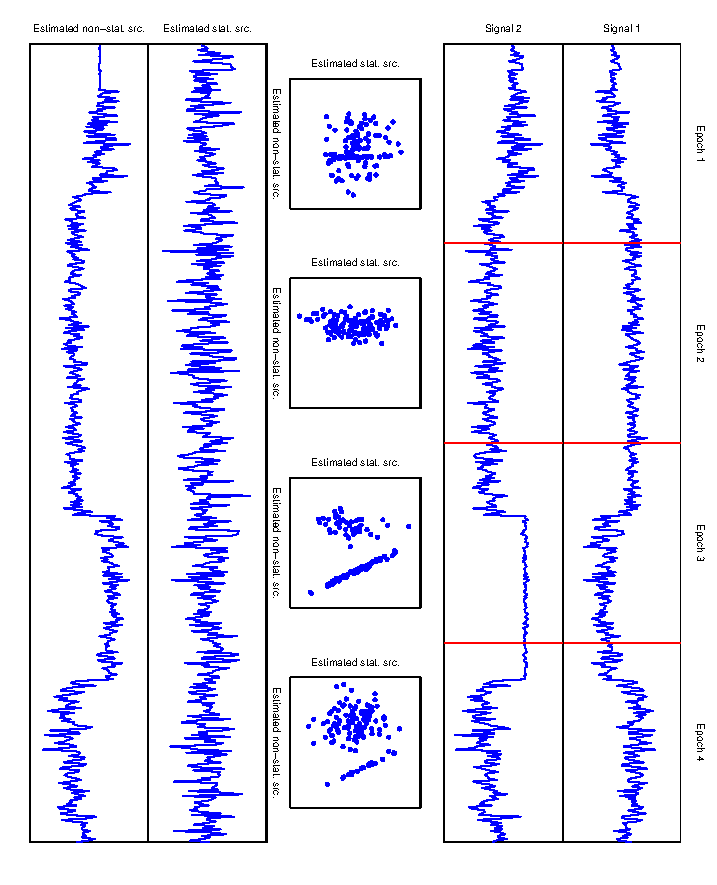
\includegraphics[angle=90,width=12.5cm]{ssa_example.pdf}
	\caption{\label{fig:matlab_example}
		Output of the Matlab example \texttt{ssa\_example.m}} 
\end{center}

The plot generated by the example script is shown in Figure~\ref{fig:matlab_example}. The top panel
shows the two dimensional input time series $x(t)$. Both dimensions (or variables, channels) appear
non-stationary. The vertical red lines indicate how the time series is segmented into four epochs. 
In the middle row, we see the result of applying SSA: for every epoch, the scatter plot shows
the distribution of the estimated stationary source (vertical axis) vs.~the estimated non-stationary 
source (horizontal axis). We can see that the mean and the variance projected to the vertical axis
is constant over the epochs, whereas both change significantly for the estimated non-stationary source. 
The bottom panel shows the time courses for the estimated stationary (top) and the estimated non-stationary 
(bottom) source. 



\end{figure}

%%%%%%%%%%%%%%%%%%%%%%%%%%%%%%%%%%%%%%%%%%%%%%%%%%%%%%%%%%%%%%%%%%%%%%%%%%%%%%%%%%%%%%%%
\FloatBarrier

\section{Frequently Asked Questions}

\paragraph{When should I use SSA?} 

SSA can be applied whenever a multivariate dataset, that has a temporal structure is conceivable 
generated as a mixture of stationary and non-stationary components, where the non-stationary 
effects are visible in changes of the mean and covariance matrix. 

\paragraph{Can I use SSA on a univariate time series?} No. 

\paragraph{How do I determine the number of stationary sources?} To date, there exists no automatic
selection procedure. In practice, one can apply SSA for several numbers of stationary sources and inspect
the result, e.g.~visually or using appropriate statistical hypothesis tests.

\paragraph{Why is it not possible to identify the non-stationary sources and what does this mean?} 
The true non-stationary sources cannot be identified because adding stationary components to a 
non-stationary time series leaves it non-stationary. This makes the estimated non-stationary sources 
arbitrary. It is therefore not possible to recover the true non-stationary sources from the mixture. 
	
\paragraph{Why is it not possible to identify the stationary subspace and what does this mean?} The basis
of the stationary subspace cannot be identified because we cannot estimate the non-stationary sources, which
are dual to the basis of the stationary subspace. If we could identify the stationary subspace, then we could
find the non-stationary sources by projecting orthogonal to it.

\paragraph{I would like to use the Toolbox from Python/Octave/or any other environment, is this possible?} 
The SSA Toolbox can be used from any environment that can invoke Java code. If you have found a way
to use the SSA Java libraries from a new programming language or environment, we would very much like
to hear from you.

\paragraph{Can I get a $p$-value for my result?} So far there is no method to establish the 
significance of the SSA solution. However, one could use a test for stationarity on the
extracted stationary sources to verify the solution, and report the corresponding $p$-values.

%%%%%%%%%%%%%%%%%%%%%%%%%%%%%%%%%%%%%%%%%%%%%%%%%%%%%%%%%%%%%%%%%%%%%%%%%%%%%%%%%%%%%%%%
\section{Developers}
\label{sec:dev}

This section contains some information about the technical structure of the SSA Toolbox
that is helpful for developers who want to extend it or use parts in other projects. The 
source code distribution of the SSA Toolbox is available from the project 
web site (see Section~\ref{sec:install_run}) and from github, a public git repository 
server, which is the primary location of the source code:
\begin{center}
	\texttt{https://github.com/paulbuenau/SSA-Toolbox}
\end{center}
On github you will always find the latest, probably unreleased version of the SSA Toolbox.

%%%%%%%%%%%%%%%%%
\subsection*{Class Structure}

The SSA Toolbox consists of the classes \texttt{SSA}, \texttt{SSAParameters}, \texttt{Data}, \texttt{Results}, \texttt{MathFunctions}, 
\texttt{GUI}, \texttt{Main}, \texttt{SSAMatrix}.

\paragraph{SSA} 

This class implements the SSA algorithm. The main-part of the implementation is in the method \texttt{optimizeOnce}, which does
the conjugate gradient descent. The calculation of the objective function and its gradient is done in the method \texttt{objectiveFunction}.
Apart from that, the class \texttt{SSA} is responsible for checking our determinacy bounds and has to throw an exception if they are violated.

\paragraph{SSAParameters}

The class \texttt{SSAParameters} stores the parameters, such as the assumed number of stationary sources, the number of restarts for the optimization and
whether to use means/covariance matrices. It is responsible to check whether the entered parameters are valid and has to throw an exception otherwise.

\paragraph{Data}

The class \texttt{Data} stores our time series and does the epochization (equally sized epochs or custom epochization). It has to check whether the
epochization is valid (and possible) and has to throw an exception otherwise.

\paragraph{Results}

This class stores the results of the SSA algorithm.

\paragraph{MathFunctions}

This class contains auxilliary functions.

\paragraph{GUI}

This class is responsible for the GUI of the standalone-version of the toolbox. It implements the interface \texttt{Logger}.

\paragraph{Main}

This is the main class of the standalone-version of the toolbox.

\paragraph{SSAMatrix}

\texttt{SSAMatrix} is a wrapper class for different matrix libraries. All matrices in the toolbox are instances of this class. It passes the
matrix operations to the currently used matrix library.

\paragraph{Logger}

This is an interface for logging. It contains only one method, which has to be implemented by all implementing classes: \texttt{appendToLog}.

\paragraph{ConsoleLogger}

This class implements the interface \texttt{Logger}. It writes all messages which are passed to the method
\texttt{appendToLog} directly to the console (needed for the matlab-wrapper).

%%%%%%%%%%%%%%%%%
\subsection*{External Dependencies}

The toolbox needs \texttt{JMatIO} (for Matlab files). The class \texttt{SSAMatrix} uses the matrix library \texttt{Colt} or \texttt{jBlas}, depending on which library
is currently selected.

%%%%%%%%%%%%%%%%%
\subsection*{Unit Tests}
The unit tests are realized using \texttt{JUnit} and can be found in the subdirectory \texttt{tests} of the repository.
There are tests for the classes \texttt{Data} and \texttt{SSA}.

\subsubsection*{Tests for the Data class}

\paragraph{\texttt{testSetNumberOfEqualSizeEpochs()}}

This test checks whether an exception is thrown if we have less data points than epochs (in case of equally sized epochs).

\paragraph{\texttt{testSetCustomEpochDefinition()}}

This test checks whether an exception is thrown if we have less data points than epochs (in case of a custom epoch definition).

\subsubsection*{Tests for the SSA class}

\paragraph{\texttt{testOptimizeMeanCov()}}

This test checks whether an exception is thrown if the determinacy bound is violated (when using both means and covariance matrices).

\paragraph{\texttt{testOptimizeMean()}}

This test checks whether an exception is thrown if the determinacy bound is violated (when using means only).

\paragraph{\texttt{testOptimizeCovariance()}}

This test checks whether an exception is thrown if the determinacy bound is violated (when using covariance matrices only).

\paragraph{\texttt{testOptimize()}}

This function contains a simple test which checks
if the SSA optimization works correctly by running the optimization on a very simple data set. This data set is $2$-dimensional, where
the first dimension is stationary and the second one is non-stationary (this means the mixing matrix to be estimated is the identity matrix).
For checking the solution of the optimization, the angle between the estimated stationary projection direction and the correct one
$\begin{pmatrix} 1 \\ 0\end{pmatrix}$ is considered. The same is done with the estimated basis vector of the non-stationary subspace,
where the correct direction is $\begin{pmatrix} 0 \\ 1\end{pmatrix}$.


%%%%%%%%%%%%%%%%%%%%%%%%%%%%%%%%%%%%%%%%%%%%%%%%%%%%%%%%%%%%%%%%%%%%%%%%%%%%%%%%%%%%%%%%
\section{Contact and Support}

If you have any question, bug report or want to discuss the application of SSA
to a specific problem, please join the SSA mailing list:
\begin{center}
        \url{http://groups.google.com/group/ssa-list}
\end{center}
You can find further
information on the official SSA homepage: 
\begin{center}
	\url{http://www.stationary-subspace-analysis.org}
\end{center}

%%%%%%%%%%%%%%%%%%%%%%%%%%%%%%%%%%%%%%%%%%%%%%%%%%%%%%%%%%%%%%%%%%%%%%%%%%%%%%%%%%%%%%%%

\bibliographystyle{plain}
\bibliography{ssa.bib}

\end{document}
